% -*- TeX-master: "../all_the_notes.tex" -*-

\section{Fabrication}
\label{sec:fabrication}

\textit{Fabrication is not an easy thing, and yet it can be completed in the space of a single
  week}

\subsection{Size parameters}\label{sec:size-parameters}
\begin{enumerate}
\item \textbf{Sample chips} are mounted in a cassette with windows. The available sizes are:

  \begin{itemize}
  \item \iunit{18}{mm} x \iunit{18}{mm};
  \item \iunit{13}{mm} x \iunit{13}{mm};
  \item \iunit{8}{mm} x \iunit{8}{mm}.
  \end{itemize}

  \begin{center}
    \includegraphics[height=5cm]{fabrication_cassette}
  \end{center}
  
  \noindent \red{\textbf{The  chip must be  larger than  this window in  order to be  fixed in
      place.}}\ec

\item \textbf{Qubit  chip}: \iunit{5}{mm} x  \iunit{3}{mm}.  This means that  a \iunit{18}{mm}
  chip will fit $ 3\times7 $ of them.

  \begin{figure}[h]
    \centering \includegraphics[height=5cm]{qubit_chip_annotated}
    \caption{\small Big markers are the P,Q markers described below.\label{fig:qubit_chip}}
  \end{figure}

  \noindent

\item \textbf{Transmission  line}: is characterized  by width  and separation with  the ground
  planes. \red{\textbf{This defines the impedance of the line, which must be 50$\Omega$}}\ec.

  \begin{itemize}
  \item \textbf{Narrow:} Width = \iunit{20}{$\mu$m}, Separation = \iunit{12}{$\mu$m};
  \item \textbf{Wide:} Width = \iunit{55}{$\mu$m}, Separation = \iunit{30}{$\mu$m}.
  \end{itemize}

   \begin{center}
     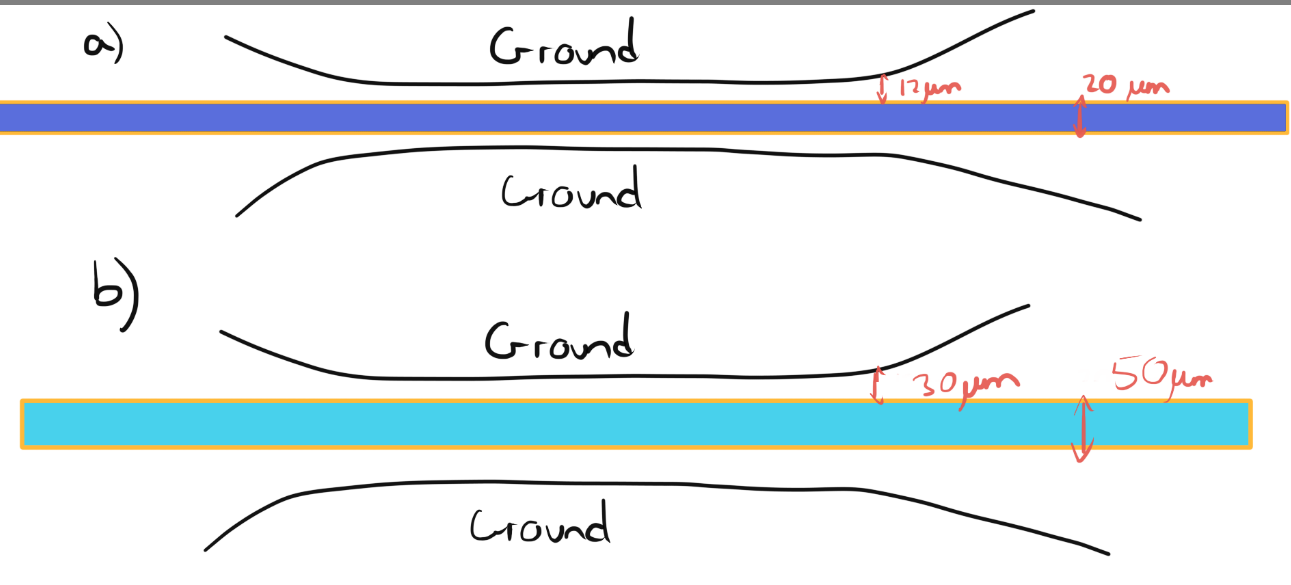
\includegraphics[height=5cm]{fab_transmission_line}
   \end{center}

 
 \end{enumerate}

 \subsection{Materials parameters}
 \label{sec:materials-parameters}

\begin{framed}\noindent 
  In  a  charge   qubit,  the  only  part   that  needs  to  be  superconducting   is  the  JJ
  superconducting-insulator-superconducting structure.  \red{\textbf{All  other components can
      be made from normal metal, as there is no persistent current.}}\ec
\end{framed}

\begin{itemize}
\item \textbf{Ground planes and bonding contacts:} Ti (\iunit{10}{nm}) - Au (\iunit{80}{nm})
\item \textbf{Aluminum JJ:}  9 degree angle evaporation of  \iunit{20}{nm} - \iunit{0.3}{mBar}
  oxidation - \iunit{30}{nm}.
\item \textbf{Aluminum }
\end{itemize}

\subsection{Structure Parameters}
\label{sec:structure-parameters}


\subsubsection{Josephson parameters (Sec.~\ref{subsec:l2-CPB})}
\label{sec:josephson-parameters}
\begin{equation}
  \label{eq:fabrication_jj_1}
  \red{E_J(1-\cos(\phi)),\qquad E_J = \frac{\Phi_0I_c}{2\pi}.}\ec
\end{equation}

\noindent and the critical current from BCS theory

\begin{equation}\label{eq:fabrication_jj_3}
  I_cR_n = \frac{\pi\Delta(0)}{2e}.
\end{equation}

\begin{framed}\noindent
  \begin{equation}\label{eq:fabrication_jj_2}
    \begin{aligned}
      E_J & = \frac{R_q}{R_n/N_{sq}}\frac{\Delta(0)}{2}\\
      R_n &= 18.4\,\text{k}\Omega \text{ for 100 } \times 100\,\text{nm}\ipow{2}
    \end{aligned}
  \end{equation}
  
  \noindent with $ R_q = \frac{h}{(2e)^2} $.  The wider  the JJ is in squares, $ N_{sq} $, the
  lower the resistance of the junction.
  
  The calibration graph for a $ 200 \times \iunit{800}{nm}^2 $ junctions is shown below:

  \ipic{4cm}{oxidation}
	
  \red{JJ  resistance  increases  by $  \sim  10\%  $  as  one  goes from  room  to  cryogenic
    temperatures.}\ec frame-contnent
\end{framed}


\subsubsection{Capacitance parameters}
\label{sec:capac-param}

\begin{equation}\label{eqn:sim_1}
  E_c = \frac{(2e)^2}{2C},
\end{equation}
 
\noindent we need the capacitance of the JJ. We  can treat the two overlapping parts of the JJ
acting a parallel plate capacitor with

\begin{framed}\noindent
  \begin{equation}\label{key}
    C = \frac{\varepsilon\varepsilon_0A}{d},
  \end{equation}
 
  \noindent with  the permittivity  for Aluminum oxide  being $ \varepsilon  \approx 10  $ and
  thickness  $  d  \approx  \iunit{2}{nm}  $.   This   give  s  a  junction  200  $  \times  $
  800\,nm\ipow{2} a charging frequency of $ E_c/\hbar \approx\iunit{19}{GHz} $.
\end{framed}

\subsubsection{Summary}
\label{sec:summary}

\begin{table}[h]
  \centering {\footnotesize
    \begin{tabular}{|c|c|p{6cm}|c|}
      \hline\textbf{Energy} &  & \textbf{Variable  parameter} &
                                                                \textbf{Energy ($ N_{sq}=10, N_{NbN} = 5$)}\\\hline
      $ E_J $ & $ \frac{R_q}{R_{\square}/N_{sq}}\frac{\Delta(0)}{2} $ & $ R_q = \frac{h}{(2e)^2} = 6.484\,\text{k}\Omega,\newline \Delta = 1.73*(k_b\times 1.3\,\text{K}) = 3.1\times10^{-23}, \newline R_\square = \iunit{18.4}{k}\Omega $ & \iunit{77.5}{GHz} \\
      $ E_C $ & $ \frac{(2e)^2}{2CN_{sq}} $ & $ \varepsilon = 10, d = \iunit{2}{nm}, \newline A = 100\times\iunit{100}{nm}^2, \newline C = \frac{\varepsilon\varepsilon_0A}{d} = \iunit{0.5}{fF} $ & \iunit{17.4}{GHz} \\
      $       E_L       $       &        $       \frac{\Phi_0^2}{(2\pi)^22LN_{NbN}}       $       &
                                                                                               $  \Phi_0 =  2\itimes{-15}\,\text{Wb}, \newline  L =
                                                                                               \iunit{1.5}{nH}
                                                                                               $
                                                                                               per
                                                                                               NbN
                                                                                               square
                                                              &
                                                                \iunit{16.2}{GHz}\\\hline
    \end{tabular}}
\end{table}
 
\subsubsection{Coupling-capacitance}
\label{sec:coupling-capacitance}

\begin{framed}\noindent
  \begin{itemize}
  \item Separation of elements should be of the order of \iunit{2}{$\mu$m};
  \item \red{\textbf{Each  \iunit{10}{$\mu$m} of  parallel structures  adds on  \iunit{1}{fF} of
        capacitance.}}\ec
  \end{itemize}

   \begin{center}
     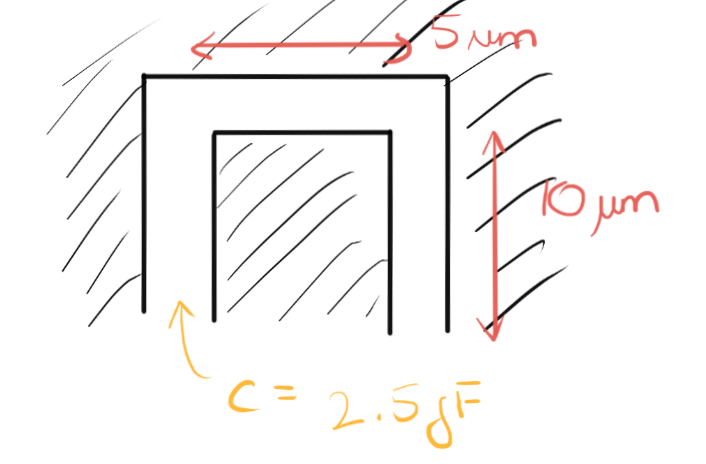
\includegraphics[height=4cm]{fab_capacitance}
     
     {\small Think  of it  as counting  the length  of the  meander between  structures.  Each
       \iunit{10}{$\mu$m} of length adds \iunit{1}{pA}.\label{fig:example-image-c}}
   \end{center}
 \end{framed}


 \subsection{Autocad-Beamer Design}
 \label{sec:autocad-design}

 \begin{itemize}
 \item All shapes \textbf{must} be polylines. They must be joined up in a single line, or they
   wont work;
 \item Units are in microns;
 \item \red{\textbf{Place  small markers in  the corners of the  pattern so that  centering is
       correct}}\ec;
 \item Once design is finished, \texttt{select all \ra  Purge \ra All \ra type "none*" \ra Yes
     to all};

 \item \red{\textbf{Decide on the P, Q markers that will be used to align the chip - note down
       their chip coordinates}}\ec
 \end{itemize}

 \subsection{Typical exposure}
 \label{sec:typic-expos-param}
 \begin{itemize}
 \item Depending on the current you'd like to use, you have to choose between:
   \begin{itemize}
   \item High Throughput: EOS mode 3, 100 keV, lens 4, from 2nA and above
   \item High Resolution: EOS mode 6, 100 keV, lens 5, 100-400 pA.
   \end{itemize}
 \item \iunit{100}{nA} for the bulky regions;
 \item \textbf{Reading markers:}
 \item Align pattern:
   \begin{enumerate}
   \item Select window to work with: A, B, C or D;
   \item Find global markers P,Q that are usually on the periphery of the chip (green)
   \item For each chip define a chip mark (blue) e.g. 490,490;
   \item Specify the center the central chip (-3500,2500)  so that the chip pattern is tied to
     the global markers.
   \end{enumerate}
   \begin{figure}[h]
     \centering \includegraphics[height=8cm]{jeol_layout}
     \caption{\small Red is  the measured values of  the P, Q markers.  Green  is the designed
       positions that are set as targets. \label{fig:jeol_layout}}
   \end{figure}
 \item
 \end{itemize}
